% =====================================================================
%  Paper draft v3 -- Indian Pines + Salinas + Pavia University results, same layout/style
%  as the supervisor's COMPAS 2024 paper.
%  Figures are read from figures/  (all already included in the package):
%     Fig_Pipeline.pdf, Fig_CNN_Architecture.pdf, Fig_Maps_IP_SA_PU.pdf
%  Red [TODO: ...] marks everything that still needs your input.
% =====================================================================
\newcommand{\CLASSINPUTtoptextmargin}{1.94cm}
\newcommand{\CLASSINPUTbottomtextmargin}{1.2cm}
\newcommand{\CLASSINPUToutersidemargin}{1.2cm}
\newcommand{\CLASSINPUTinnersidemargin}{1.5cm}

\documentclass[conference]{IEEEtran}

\usepackage{cite}
\usepackage{amsmath,amssymb,amsfonts}
\usepackage{graphicx}
\usepackage{textcomp}
\usepackage{xcolor}
\usepackage{comment}
\usepackage{float}
\usepackage{multirow}
\usepackage{booktabs}
\usepackage{array}
\usepackage[T1]{fontenc}
\usepackage{mathptmx}
\usepackage{subcaption}
\usepackage{hyperref}
\hypersetup{colorlinks=true, linkcolor=black, citecolor=black, filecolor=black, urlcolor=black}

\graphicspath{{figures/}{./}}

% ---- helpers -------------------------------------------------------
\newcommand{\todo}[1]{{\color{red}[TODO: #1]}}

\def\BibTeX{{\rm B\kern-.05em{\sc i\kern-.025em b}\kern-.08em
		T\kern-.1667em\lower.7ex\hbox{E}\kern-.125emX}}

\IEEEoverridecommandlockouts

\begin{document}
	
	\title{Compact Relevance-Graded 3D-2D CNN with Attention for Hyperspectral Image Classification using Segmented PCA, mRMR and Metaheuristic Feature Selection}
	
	\author{\IEEEauthorblockN{\todo{Your Name}}
		\IEEEauthorblockA{\textit{Computer Science and Engineering} \\
			\textit{Varendra University}\\
			Rajshahi, Bangladesh \\
			\todo{your email}}
		\and
		\IEEEauthorblockN{Your Name}
		\IEEEauthorblockA{\textit{Computer Science and Engineering} \\
			\textit{Varendra University}\\
			Rajshahi, Bangladesh \\
			your email}
	}
	
	\maketitle
	
	\begin{abstract}
		Hyperspectral image (HSI) classification with deep networks is hindered by high spectral dimensionality, redundant bands and a small number of labelled samples. This paper presents a compact framework that combines Segmented PCA (Seg-PCA), minimum-Redundancy-Maximum-Relevance (mRMR) ranking and a metaheuristic subset search to reduce the 200 (Indian Pines), 204 (Salinas) and 103 (Pavia University) spectral bands to only five, four and seven input features. The selected features are split into three relevance groups, and each group is processed by its own 3D-2D CNN stream: the most relevant group gets the deepest stream and the largest kernel. The stream outputs are fused, refined with a convolutional block attention module (CBAM) and classified through global average pooling. With 16\% of the labelled pixels used for training, the model reaches an overall accuracy of 98.92\% $\pm$ 0.24, 99.94\% $\pm$ 0.03 and 99.47\% $\pm$ 0.07 on the three datasets (mean of five seeds) with fewer than 79,000 parameters. This is comparable to earlier methods that use 15 features on Indian Pines and Salinas, and 0.15--0.47 points lower than the strongest prior result on Pavia University. An ablation study shows that the global-average-pooling head matches a flatten head with about 17 times fewer parameters on Indian Pines and Salinas, but loses 0.43 points on Pavia University, while the accuracy changes caused by the other components stay close to the seed-to-seed variation.
	\end{abstract}
	
	\begin{IEEEkeywords}
		Hyperspectral Image, Segmented PCA, mRMR, Metaheuristic Feature Selection, 3D-2D CNN, CBAM.
	\end{IEEEkeywords}
	
	% =====================================================================
	\section{Introduction}
	% =====================================================================
	Hyperspectral remote sensing records hundreds of narrow spectral bands for every pixel, so each image is a data cube with two spatial and one spectral dimension. The spectral signature carries information about the chemical and physical structure of the observed material, which makes HSI useful for mineral exploration, environmental monitoring, precision agriculture and food quality assurance. Deep learning has become the main tool for HSI analysis, with convolutional neural networks (CNN)\cite{cnn14}, stacked autoencoders (SAE)\cite{sae8}, recurrent neural networks (RNN)\cite{rnn16} and generative adversarial networks\cite{gan19} all applied to the task.
	
	Many works combine spatial and spectral information. A 2D CNN extracts spatial features efficiently\cite{makantis}, while 3D CNNs process the spatial and spectral dimensions together with a smaller number of parameters\cite{Hamida}. Fast 3D-CNN\cite{compact} uses incremental PCA together with a 3D-2D CNN, and HybridSN\cite{hybridsn} stacks 3D and 2D convolutions to learn spectral-spatial features. Other designs extract the spectral and spatial features separately and then fuse them\cite{guo,li}, and a wavelet-based Spectral Network has also been proposed\cite{spectral}. Multibranch fusion of 2D and 3D CNNs\cite{multibranch} improves accuracy 
	over single-path networks, and adding a segmentation step before fusion 
	further boosts performance\cite{multibranch2}. On the preprocessing side, segmented versions of PCA\cite{spca}, t-SNE\cite{stsne} and NMF\cite{snmf} better respect the local structure of correlated spectral bands.
	
	In an earlier work\cite{ahmed2024}, Seg-PCA and mRMR were used to rank 
	15 features, which were split into three equal groups and fed to a 
	three-branch 2D-3D CNN. That design still keeps 15 features and ends in a 
	flatten layer followed by fully connected layers. In this paper we extend it in three ways. First, a binary metaheuristic searches the 15 ranked features for a much smaller subset, with a fitness that rewards accuracy and penalises subset size. Second, every stream gets a residual shortcut with a separable 2D convolution, and the fused features are refined by CBAM\cite{cbam}. Third, a global average pooling (GAP) head replaces the flatten layer, which keeps the model small.
	
	The main contributions of this paper are:
	\begin{enumerate}
		\item A three-step feature pipeline (Seg-PCA, mRMR and a metaheuristic subset 
		search) that reduces the 200, 204 and 103 spectral bands of Indian Pines, 
		Salinas and Pavia University to only 5, 4 and 7 input features—an overall 
		reduction of 97.5\%, 98.0\% and 93.2\%.
		\item A relevance-graded three-stream 3D-2D CNN with residual shortcuts, CBAM and a GAP head, with fewer than 79,000 trainable parameters.
		\item A five-seed ablation study on the three datasets covering the pipeline stages, the pooling head, the kernel design, the CBAM components and five metaheuristic optimizers, reported with mean and standard deviation.
	\end{enumerate}
	
	The rest of the paper is organised as follows. Section~\ref{related_theory} gives the related theory, Section~\ref{Proposed} describes the proposed method, Section~\ref{experiment} reports the experiments and Section~\ref{conclusion} concludes the paper.
	
	% =====================================================================
	\section{Related Theory} \label{related_theory}
	% =====================================================================
	
	\subsection{Convolutional Block Attention Module}
	CBAM\cite{cbam} refines a feature map $F$ in two steps. Channel attention decides \textit{what} is important and spatial attention decides \textit{where} it is important:
	\begin{equation}
		M_c(F)=\sigma\big(W_2\,\delta(W_1\,\mathrm{GAP}(F))+W_2\,\delta(W_1\,\mathrm{GMP}(F))\big),
	\end{equation}
	\begin{equation}
		M_s(F')=\sigma\big(f^{7\times7}([\mathrm{Avg}_c(F');\mathrm{Max}_c(F')])\big),
	\end{equation}
	where $\delta$ is ReLU, $\sigma$ is the sigmoid, $W_1,W_2$ are shared dense layers, and $\mathrm{Avg}_c,\mathrm{Max}_c$ are the channel-wise mean and maximum maps.
	
	\subsection{Metaheuristic Feature Selection}
	Feature selection with $n$ candidate features has $2^n$ possible subsets, so exhaustive search is impossible for large $n$. Metaheuristics search this space with a population of candidate solutions. In the binary version, each candidate is a mask in which 1 means the feature is kept. Common choices are Particle Swarm Optimization (PSO)\cite{pso}, Grey Wolf Optimizer (GWO)\cite{gwo}, Genetic Algorithm (GA)\cite{ga}, Differential Evolution (DE)\cite{de} and Moth-Flame Optimization (MFO)\cite{mfo}. All five are compared in this work.
	
	% =====================================================================
	\section{Proposed Methodology}\label{Proposed}
	% =====================================================================
	The proposed framework has five stages: data splitting, Seg-PCA, two-step feature selection, patch extraction and a relevance-graded 3D-2D CNN with attention. Fig.~\ref{pipeline} shows the full pipeline and Fig.~\ref{cnn} shows the network.
	
	\begin{figure*}[t]
		\centering
		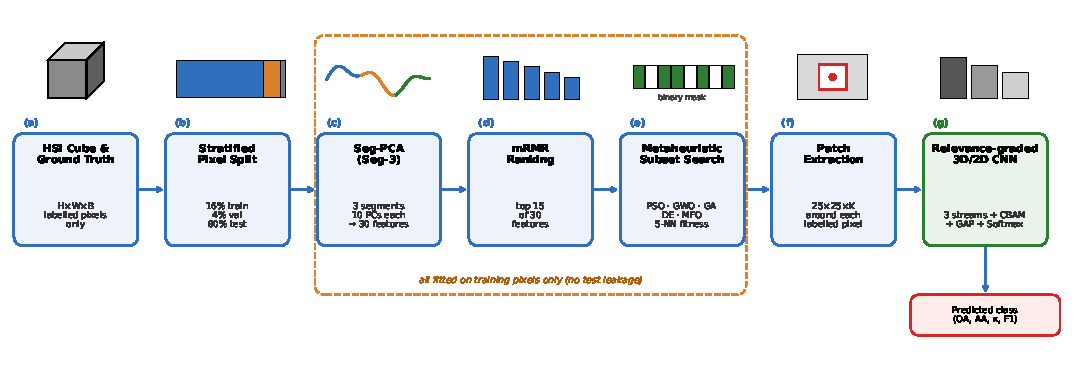
\includegraphics[width=0.95\textwidth]{Fig_Pipeline.pdf}
		\caption{Overview of the proposed pipeline. Seg-PCA, mRMR and the metaheuristic search are fitted on training pixels only. (a)~Hyperspectral cube with ground truth; (b)~stratified 16/4/80 split; (c)~segmented PCA; (d)~mRMR ranking; (e)~binary-mask subset search; (f)~patch extraction; (g)~relevance-graded 3D-2D CNN.}
		\label{pipeline}
	\end{figure*}
	
	\subsection{Data Splitting}
	The labelled pixels are divided by stratified random sampling into 16\% training, 4\% validation and 80\% test pixels. This follows the ``20\%'' protocol of the earlier work\cite{ahmed2024}, in which 20\% of the data is used for training and one fifth of it is kept for validation, so the results can be compared directly. Only pixel indices are split. Every transform below (scaling, PCA, feature selection) is fitted on training pixels only, so no test information leaks into training.
	
	\subsection{Segmented PCA (Seg-PCA)}
	Neighbouring bands are strongly correlated, while distant bands are not. A single PCA over all bands mixes these regions, so the spectrum is first divided into $L=3$ continuous segments of highly correlated bands, as in\cite{ahmed2024}. For segment $t$, the bands $\mathbf{D}_t$ are scaled and projected:
	\begin{equation}
		\mathbf{Z}_t = \mathrm{PCA}_t\big(\mathrm{MinMax}_t(\mathbf{D}_t)\big),\quad t=1,2,3,
	\end{equation}
	and the first 10 components of every segment are kept. Joining the three outputs gives a 30-dimensional vector for each pixel. The scaler and PCA of every segment are fitted on training pixels only. Table~\ref{segtable} lists the segments of the three datasets together with the average band-to-band correlation inside each segment.
	
	\begin{table}[t]
		\centering
		\caption{Seg-PCA segments (Seg-3) of the three datasets. Var. is the explained variance of the 10 kept components.}
		\label{segtable}
		\footnotesize
		\setlength{\tabcolsep}{1.8pt}
		\begin{tabular}{@{}llcccc@{}}
			\toprule
			Dataset & Seg. & Bands & Count & Avg. corr. & Var. (\%) \\ \midrule
			\multirow{3}{*}{Indian Pines} & Seg-1 & 1--36    & 36 & 0.873 & 98.83 \\
			& Seg-2 & 37--102  & 66 & 0.546 & 95.37 \\
			& Seg-3 & 103--200 & 98 & 0.950 & 99.38 \\ \midrule
			\multirow{3}{*}{Salinas}      & Seg-1 & 1--36    & 36 & 0.919 & 99.96 \\
			& Seg-2 & 37--106  & 70 & 0.820 & 99.98 \\
			& Seg-3 & 107--204 & 98 & 0.972 & 99.90 \\ \midrule
			\multirow{3}{*}{Pavia Univ.} & Seg-1 & 1--37    & 37 & 0.972 & 99.93 \\
			& Seg-2 & 38--72   & 35 & 0.946 & 99.98 \\
			& Seg-3 & 73--103  & 31 & 0.953 & 99.97 \\ \bottomrule
		\end{tabular}
	\end{table}
	
	\subsection{Feature Selection}
	Selection has two steps, so that we get both a good ranking and a small final subset.
	
	\subsubsection{mRMR Ranking}
	mRMR\cite{mrmr} prefers features that are strongly related to the class label but not related to each other. With mutual information $M(\cdot;\cdot)$, a feature set $S$ and the class $c$, relevance and redundancy are
	\begin{equation}
		R_e=\frac{1}{|S|}\sum_{b_i\in S}M(b_i;c),\qquad
		R_d=\frac{1}{|S|^2}\sum_{b_i,b_j\in S}M(b_i;b_j),
	\end{equation}
	and features are ranked by maximising $R_e-R_d$. The top 15 of the 30 Seg-PCA features are kept in ranked order. For Indian Pines the best-ranked features come mostly from Seg-3 (S3\_PC1, S3\_PC2, S3\_PC9), for Salinas from Seg-1 (S1\_PC1, S1\_PC2, S1\_PC5) and for Pavia University also from Seg-1 (S1\_PC1, S1\_PC2, S1\_PC6).
	
	\subsubsection{Metaheuristic Subset Search}
	From the 15 ranked features, a binary metaheuristic searches for the best subset. We compare PSO, GWO, GA, DE and MFO. All use a population of 25 and 20 iterations. The fitness, to be minimised, is
	\begin{equation}
		f(\mathbf{m})=\alpha\,(1-\mathrm{BA})+(1-\alpha)\,\frac{|F_{sel}|}{|F_{all}|},
	\end{equation}
	where BA is the balanced accuracy of a distance-weighted 5-NN classifier from 3-fold stratified cross-validation on the training set, $|F_{sel}|/|F_{all}|$ is the fraction of kept features and $\alpha=0.95$. The mask of the algorithm with the lowest fitness gives the final subset. In our runs DE gave the lowest fitness on Indian Pines and Salinas and kept five and four features. On Pavia University DE and PSO tie at a fitness of 0.2060 with seven 
	features each; because we iterate the optimizers in a fixed order 
	(PSO, GWO, GA, DE, MFO), the earliest one (PSO) is selected for the 
	final model (Table~\ref{metatable}).
	
	\subsection{Patch Extraction}
	The trained Seg-PCA transforms are applied to every pixel and only the selected features are kept, giving a cube of size $X\times Y\times K$. Around every labelled pixel a $25\times25\times K$ patch is cut, with zero padding at the image border so that the labelled pixel is always at the centre. The label of a patch is the label of its centre pixel.
	
	\subsection{Relevance-Graded 3D-2D CNN}
	\begin{figure*}[t]
		\centering
		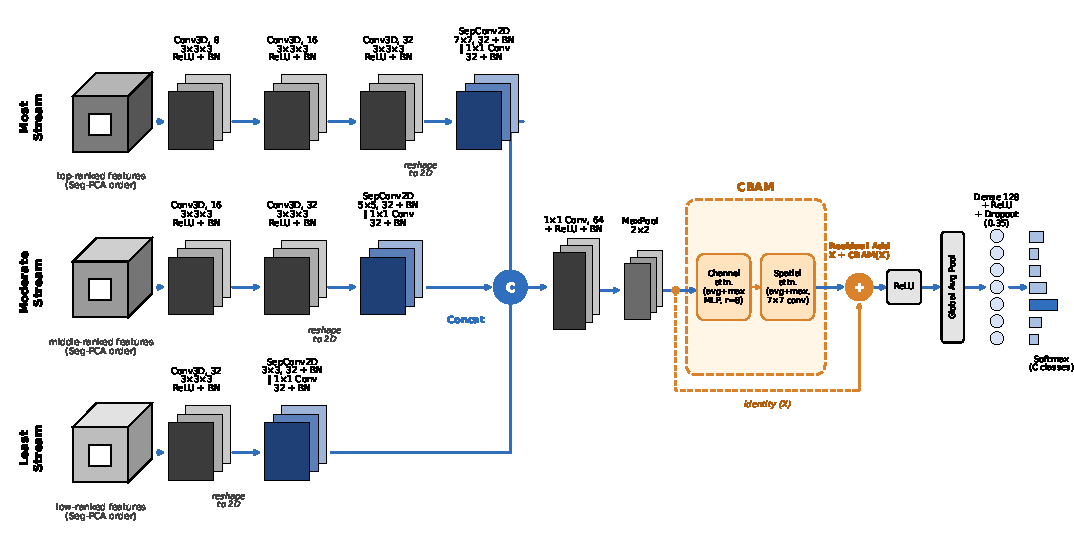
\includegraphics[width=\textwidth]{Fig_CNN_Architecture.pdf}
		\caption{Architecture of the relevance-graded 3D-2D CNN. The selected features are split into Most, Moderate and Least relevant groups. Each group goes through its own stream (Conv3D layers with ReLU and BN, then a separable 2D convolution in parallel with a $1\times1$ convolution, both followed by BN). The three stream outputs are concatenated, projected by a $1\times1$ convolution, pooled, and refined by CBAM. The CBAM output is added to its input (residual add) and passed through ReLU, followed by GAP, a dense layer with ReLU and dropout, and softmax.}
		\label{cnn}
	\end{figure*}
	
	\subsubsection{Relevance Groups}
	Features with a higher mRMR rank carry more class information, so they should get a stronger branch. The selected features are divided into three groups of nearly equal size in mRMR order: \textit{Most}, \textit{Moderate} and \textit{Least} relevant. In our runs the groups have 2, 2 and 1 features for Indian Pines, 2, 1 and 1 for Salinas and 3, 2 and 2 for Pavia University. Inside each group the channels are put back in their original Seg-PCA order, because a 3D convolution assumes that neighbouring channels are related.
	
	\subsubsection{Three-Stream Design}
	Every group has its own stream. The more relevant the group, the deeper its 3D part and the larger its 2D kernel: the Most stream has three Conv3D layers (8, 16 and 32 filters) and a $7\times7$ kernel, the Moderate stream has two (16 and 32 filters) and a $5\times5$ kernel, and the Least stream has one (32 filters) and a $3\times3$ kernel (Fig.~\ref{cnn}). In a stream, the input passes through $3\times3\times3$ Conv3D layers, each followed by ReLU and batch normalisation (BN). The 3D output is reshaped into a 2D map by merging the spectral and filter dimensions. A separable 2D convolution (32 filters, stream kernel size, ReLU) followed by BN is then applied. A parallel $1\times1$ convolution (32 filters, ReLU, BN) works as a shortcut, and its output is concatenated with the separable convolution output.
	
	
	\subsubsection{Fusion, Attention and Classification}
	The three stream outputs (each with 64 channels after concatenation with the shortcut) are concatenated, projected by a $1\times1$ convolution with 64 filters, ReLU and BN, and reduced by $2\times2$ max pooling from $25\times25$ to $12\times12$. CBAM\cite{cbam} then applies channel attention (reduction ratio 8) followed by spatial attention ($7\times7$ convolution). If $F$ is the CBAM input, the attended map is $F''=M_s(F')\otimes F'$ with $F'=M_c(F)\otimes F$, and the output is $\mathrm{ReLU}(F+F'')$. Global average pooling\cite{nin} turns the map into a 64-dimensional vector, followed by a dense layer of 128 units with ReLU, dropout (0.35) and a softmax layer. Compared with flattening, GAP greatly reduces the number of parameters and the risk of overfitting. In total the network has 73,707 parameters for Indian Pines, 70,859 for Salinas and 78,756 for Pavia University.
	
	% =====================================================================
	\section{Experimental Result and Analysis} \label{experiment}
	% =====================================================================
	\subsection{Datasets and Experimental Setup}
	We use the Indian Pines (IP), Salinas (SA) and Pavia University (PU) datasets, all publicly available. IP has $145\times145$ pixels, 200 bands after removing the water-absorption bands, 16 classes and 10,249 labelled pixels (8,200 for testing). SA has $512\times217$ pixels, 204 bands after removing 20 such bands, 16 classes and 54,129 labelled pixels (43,304 for testing). PU has $610\times340$ pixels, 103 bands, 9 classes and 42,776 labelled pixels (34,221 for testing). In IP some classes are very small; for example, Oats has only 3 and Grass-pasture-mowed only 5 training pixels, while SA and PU have much larger classes.
	
	The network is implemented in TensorFlow 2.21.0 and trained on a single NVIDIA T4 GPU in Google Colab. We use the Adam optimiser\cite{adam} with a learning rate of $5\times10^{-4}$, a batch size of 64 and at most 100 epochs. Categorical cross-entropy with label smoothing of 0.05\cite{labelsmooth} is used. Because the classes are unbalanced, class weights are computed from the inverse class frequency and softened with a power of 0.5. L2 regularisation ($10^{-5}$) is applied to the dense and separable convolution weights, and no data augmentation is used. The learning rate is halved if the validation loss does not improve for 6 epochs, and training stops if the validation accuracy does not improve for 15 epochs, restoring the best weights. The window size is $25\times25$. We report Overall Accuracy (OA), Average Accuracy (AA), Kappa coefficient and macro F1-score on the test set. To check stability, every model is trained with five seeds (42, 123, 456, 789, 1011) and we report the mean and the population standard deviation. The seeds change the network initialisation and batch order only; the data split and the selected features stay fixed.
	
	\subsection{Findings of the Experiments}
	
	\subsubsection{Feature Selection}
	Table~\ref{metatable} compares the five optimizers. DE gives the lowest fitness on Indian Pines and Salinas, with five and four features. On Pavia University, DE and PSO tie at a fitness of 0.2060 with seven features each, and PSO was used for the final model. The selection is cheap: the optimizer of the final model needs 6.89 s on IP, 30.98 s on SA and 54.17 s on PU, and mRMR needs 5.19 s, 6.18 s and 4.80 s, compared with 176.5 s, 315.7 s and 605.8 s to train the network once. The table also shows the CNN accuracy obtained with each subset. The lowest fitness does not give the highest CNN accuracy: on IP, GWO keeps eight features and reaches 99.27\%, while DE reaches 98.94\%. On SA and PU all five optimizers are within 0.02 and 0.06 points of each other, so on these datasets the choice of optimizer hardly matters. The 5-NN fitness is therefore only a rough proxy for the final CNN, and the benefit of the subset search is mainly the smaller input and model.
	
	\begin{table*}[t]
		\centering
		\caption{Metaheuristic selection on the 15 mRMR features. $F$ is the number of selected features and OA is the mean $\pm$ std (\%) of five CNN runs with the selected subset. $^{\dagger}$ marks the subset used in the final model.}
		\label{metatable}
		\footnotesize
		\setlength{\tabcolsep}{4pt}
		\begin{tabular}{@{}lccc@{\hspace{14pt}}ccc@{\hspace{14pt}}ccc@{}}
			\toprule
			& \multicolumn{3}{c}{Indian Pines} & \multicolumn{3}{c}{Salinas} & \multicolumn{3}{c}{Pavia University} \\ \cmidrule(r){2-4}\cmidrule(r){5-7}\cmidrule{8-10}
			Optimizer & Fitness & $F$ & OA & Fitness & $F$ & OA & Fitness & $F$ & OA \\ \midrule
			DE  & \textbf{0.3495}$^{\dagger}$ & 5 & 98.94 $\pm$ 0.32 & \textbf{0.0736}$^{\dagger}$ & 4 & 99.94 $\pm$ 0.02 & \textbf{0.2060} & 7 & \textbf{99.55 $\pm$ 0.08} \\
			PSO & 0.3519 & 4 & 99.10 $\pm$ 0.18 & 0.0756 & 5 & 99.94 $\pm$ 0.03 & \textbf{0.2060}$^{\dagger}$ & 7 & 99.49 $\pm$ 0.05 \\
			MFO & 0.3597 & 4 & 99.07 $\pm$ 0.14 & 0.0768 & 4 & 99.94 $\pm$ 0.05 & 0.2107 & 8 & 99.49 $\pm$ 0.08 \\
			GWO & 0.3809 & 8 & \textbf{99.27 $\pm$ 0.07} & 0.0757 & 5 & \textbf{99.96 $\pm$ 0.03} & 0.2080 & 10 & 99.53 $\pm$ 0.16 \\
			GA  & 0.4057 & 8 & 82.44 $\pm$ 33.08$^{*}$ & 0.0816 & 8 & 99.95 $\pm$ 0.03 & 0.2129 & 7 & 99.50 $\pm$ 0.06 \\ \bottomrule
		\end{tabular}\\[3pt]
		{\scriptsize $^{*}$One of five seeds did not converge (OA 16.29\%); the other four give 98.57--99.24\%.}
	\end{table*}
	
	\subsubsection{Classification Results}
	Table~\ref{results} gives the main results, which are the mean and standard deviation over the five seeds: 98.92\% OA on Indian Pines, 99.94\% on Salinas and 99.47\% on Pavia University. The AA on IP varies more than the OA (97.92\% $\pm$ 0.96) because the rare classes, which have only a few training pixels, depend on the initialisation; the lowest AA, 96.24\%, comes from seed 789. The run used for the maps in Fig.~\ref{maps} (the main run) reaches 99.23\% OA, 99.16\% AA and a Kappa of 0.9912 on IP, 99.90\%, 99.90\% and 0.9989 on SA, and 99.57\%, 99.12\% and 0.9943 on PU. We use the five-seed mean as the main result, because a single run can be better or worse than the average. In the main runs all classes have a recall of at least 95.95\% on IP (lowest for Stone-Steel-Towers) and 99.42\% on SA (lowest for Lettuce-romaine-7wk). On PU all classes except Shadows have a recall of at least 98.57\% (lowest for Gravel), while Shadows, the smallest class (758 test pixels), has a recall of 96.57\% and a precision of 94.70\%.
	
	\begin{table}[t]
		\centering
		\caption{Results of the proposed model (16\% training), mean $\pm$ std of five seeds}
		\label{results}
		\renewcommand*\arraystretch{1.1}
		\footnotesize
		\setlength{\tabcolsep}{3pt}
		\begin{tabular}{@{}lcccc@{}}
			\toprule
			Dataset & OA (\%) & AA (\%) & Kappa & Macro F1 (\%) \\ \midrule
			Indian Pines & 98.92 $\pm$ 0.24 & 97.92 $\pm$ 0.96 & 0.9877 $\pm$ 0.0028 & 98.21 $\pm$ 0.60 \\
			Salinas      & 99.94 $\pm$ 0.03 & 99.93 $\pm$ 0.04 & 0.9993 $\pm$ 0.0003 & 99.92 $\pm$ 0.04 \\
			Pavia Univ.  & 99.47 $\pm$ 0.07 & 98.59 $\pm$ 0.21 & 0.9929 $\pm$ 0.0009 & 98.70 $\pm$ 0.18 \\ \bottomrule
		\end{tabular}
	\end{table}
	
	\begin{figure*}[t]
		\centering
		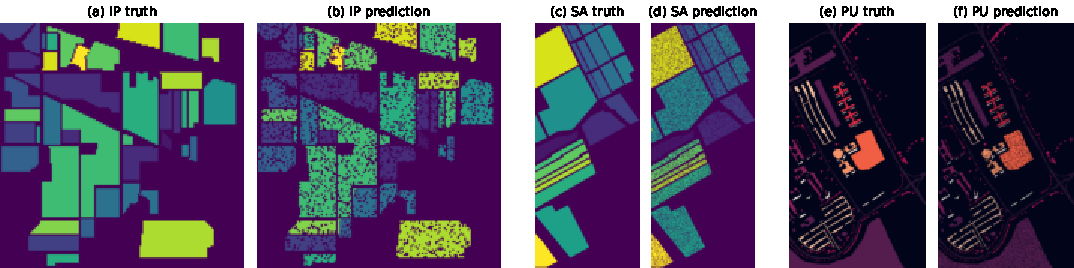
\includegraphics[width=\textwidth]{Fig_Maps_IP_SA_PU.pdf}
		\caption{Ground truth and prediction of the main run on the held-out test pixels (the other pixels are shown as background) for Indian Pines (IP, a--b), Salinas (SA, c--d) and Pavia University (PU, e--f).}
		\label{maps}
	\end{figure*}
	
	\subsubsection{Comparison with Other Methods}
	Table~\ref{stateofarts} compares the proposed model with the methods of the earlier paper\cite{ahmed2024}. The rows of the other methods are taken from\cite{ahmed2024}, where all 
	of them were run with 15 input features on the 20\% training split. On Indian Pines the five-seed mean OA of the proposed model (98.92\%) is above the 2D-3D multibranch network\cite{multibranch} (98.67\%), 0.17 points below HybridSN\cite{hybridsn} (99.09\%) and 0.20 points below the earlier model\cite{ahmed2024} (99.12\%). Its AA (97.92\%) is lower than both of these (98.35\% and 99.35\%). On Salinas the OA (99.94\%) is 0.03 points below HybridSN and the multibranch network (99.97\%) and 0.06 points below the earlier model (100\%). On IP and SA these differences are within the seed-to-seed variation of our model or very small. On Pavia University the OA (99.47\%) equals that of Fast Compact 3D CNN\cite{compact} (99.46\%) but is 0.15, 0.41 and 0.47 points below the multibranch network (99.62\%), HybridSN (99.88\%) and the earlier model (99.94\%). These gaps are two to six times the seed-to-seed standard deviation (0.07), so on PU the compact model is less accurate than the 15-feature models. We therefore do not claim that the proposed model is more accurate. Its benefit is that it is comparable on IP and SA with one third and one quarter of the input features, and it uses less than half of the features on PU (7 of 15). Note that our values are means over five seeds, while the values of the other methods come from the earlier paper.
	
	\begin{table}[t]
		\centering
		\caption{Comparison (16\% training, 4\% validation, 80\% test). The 
			rows of the other methods are taken from\cite{ahmed2024}, where all 
			of them were run with 15 input features (Feat.) on the 20\% training 
			split.}
		\label{stateofarts}
		\renewcommand*\arraystretch{1.05}
		\footnotesize
		\setlength{\tabcolsep}{3pt}
		\begin{tabular}{@{}llcccc@{}}
			\toprule
			Dataset & Model & Feat. & OA (\%) & AA (\%) & Kappa (\%) \\ \midrule
			\multirow{6}{*}{IP}
			& 2D CNN\cite{makantis}               & 15 & 53.54 & 71.65 & 51.25 \\
			& Fast Compact 3D CNN\cite{compact}   & 15 & 83.39 & 61.03 & 80.95 \\
			& HybridSN\cite{hybridsn}             & 15 & 99.09 & 98.35 & 98.96 \\
			& 2D-3D Multibranch\cite{multibranch} & 15 & 98.67 & 98.35 & 98.48 \\
			& Ahmed \textit{et al.}\cite{ahmed2024} & 15 & 99.12 & 99.35 & 99.00 \\
			& \textbf{Proposed}                   & 5  & 98.92 $\pm$ 0.24 & 97.92 & 98.77 \\ \midrule
			\multirow{6}{*}{SA}
			& 2D CNN\cite{makantis}               & 15 & 85.65 & 95.52 & 84.19 \\
			& Fast Compact 3D CNN\cite{compact}   & 15 & 98.76 & 97.35 & 98.62 \\
			& HybridSN\cite{hybridsn}             & 15 & 99.97 & 99.93 & 99.97 \\
			& 2D-3D Multibranch\cite{multibranch} & 15 & 99.97 & 99.96 & 99.97 \\
			& Ahmed \textit{et al.}\cite{ahmed2024} & 15 & 100   & 100   & 99.99 \\
			& \textbf{Proposed}                   & 4  & 99.94 $\pm$ 0.03 & 99.93 & 99.93 \\ \midrule
			\multirow{6}{*}{PU}
			& 2D CNN\cite{makantis}               & 15 & 94.46 & 94.68 & 92.71 \\
			& Fast Compact 3D CNN\cite{compact}   & 15 & 99.46 & 99.12 & 99.28 \\
			& HybridSN\cite{hybridsn}             & 15 & 99.88 & 99.76 & 99.84 \\
			& 2D-3D Multibranch\cite{multibranch} & 15 & 99.62 & 99.54 & 99.49 \\
			& Ahmed \textit{et al.}\cite{ahmed2024} & 15 & 99.94 & 99.93 & 99.93 \\
			& \textbf{Proposed}                   & 7  & 99.47 $\pm$ 0.07 & 98.59 & 99.29 \\ \bottomrule
		\end{tabular}
	\end{table}
	
	\subsubsection{Ablation Study}
	Table~\ref{ablation} adds the pipeline components one by one, and Table~\ref{ablation2} compares the pooling head, the kernel design, the CBAM components and the input features. Each variant is trained with the same five seeds on all three datasets. The full list of variants, with AA, features and parameters, is given in the supplementary table. Stages 0--4 use plain MinMax scaling and 12 PCA components, Stage 5 uses the 15 Seg-PCA/mRMR features and Stage 6 uses the subset chosen by the metaheuristic search (5, 4 and 7 features for IP, SA and PU).
	
	\begin{table}[t]
		\centering
		\caption{Stage-wise ablation, OA (\%) as mean $\pm$ std of five seeds. Stage 6 is the proposed model.}
		\label{ablation}
		\renewcommand*\arraystretch{1.05}
		\footnotesize
		\setlength{\tabcolsep}{1.8pt}
		\begin{tabular}{@{}lccc@{}}
			\toprule
			Variant & IP & SA & PU \\ \midrule
			0: Single-scale & 98.72 $\pm$ 0.35 & 99.95 $\pm$ 0.02 & 99.50 $\pm$ 0.11 \\
			1: + Multi-scale & 99.16 $\pm$ 0.22 & 99.97 $\pm$ 0.01 & 99.72 $\pm$ 0.08 \\
			2: + Residual & 99.15 $\pm$ 0.16 & 99.96 $\pm$ 0.02 & 99.68 $\pm$ 0.07 \\
			3: + Graded streams & 98.93 $\pm$ 0.40 & 99.93 $\pm$ 0.03 & 99.65 $\pm$ 0.05 \\
			4: + CBAM & 99.16 $\pm$ 0.19 & 99.94 $\pm$ 0.03 & 99.45 $\pm$ 0.05 \\
			5: + Seg-PCA, mRMR & 99.07 $\pm$ 0.16 & 99.96 $\pm$ 0.03 & 99.60 $\pm$ 0.04 \\
			6: + Subset (proposed) & 98.94 $\pm$ 0.32 & 99.94 $\pm$ 0.02 & 99.49 $\pm$ 0.05 \\ \\ \bottomrule
		\end{tabular}
	\end{table}
	
	\begin{table}[t]
		\centering
		\caption{Head, kernel, CBAM and input-feature ablation, OA (\%) as mean $\pm$ std of five seeds.}
		\label{ablation2}
		\renewcommand*\arraystretch{1.05}
		\footnotesize
		\setlength{\tabcolsep}{1.8pt}
		\begin{tabular}{@{}lccc@{}}
			\toprule
			Variant & IP & SA & PU \\ \midrule
			\textbf{Proposed (GAP head)} & 98.94 $\pm$ 0.32 & 99.94 $\pm$ 0.02 & 99.49 $\pm$ 0.05 \\
			GMP head & 98.73 $\pm$ 0.13 & 99.92 $\pm$ 0.05 & 99.35 $\pm$ 0.14 \\
			Flatten head & 98.84 $\pm$ 0.09 & 99.97 $\pm$ 0.01 & 99.92 $\pm$ 0.03 \\
			\midrule
			No residual shortcut & 99.14 $\pm$ 0.14 & 99.93 $\pm$ 0.05 & 99.61 $\pm$ 0.04 \\
			Uniform 7$\times$7 kernel & 84.71 $\pm$ 28.66$^{*}$ & 99.96 $\pm$ 0.04 & 99.54 $\pm$ 0.09 \\
			Reversed kernels (3/5/7) & 99.20 $\pm$ 0.07 & 99.92 $\pm$ 0.04 & 99.49 $\pm$ 0.09 \\
			Single stream (7/5/3) & 99.08 $\pm$ 0.20 & 99.94 $\pm$ 0.02 & 99.61 $\pm$ 0.05 \\
			\midrule
			CBAM: channel only & 99.05 $\pm$ 0.31 & 99.90 $\pm$ 0.05 & 99.48 $\pm$ 0.09 \\
			CBAM: spatial only & 98.98 $\pm$ 0.13 & 99.96 $\pm$ 0.03 & 99.69 $\pm$ 0.03 \\
			CBAM: no residual add & 98.97 $\pm$ 0.14 & 99.91 $\pm$ 0.04 & 99.50 $\pm$ 0.04 \\
			\midrule
			Input: 12 PCA & 99.16 $\pm$ 0.23 & 99.97 $\pm$ 0.02 & 99.48 $\pm$ 0.04 \\
			Input: 15 mRMR & 98.98 $\pm$ 0.19 & 99.96 $\pm$ 0.02 & 99.60 $\pm$ 0.05 \\ \\ \bottomrule
		\end{tabular}\\[3pt]
		{\scriptsize $^{*}$The large std shows that at least one seed did not converge.}
	\end{table}
	
	The three datasets behave differently. On Salinas every variant reaches 99.90--99.97\% OA with a standard deviation of at most 0.05, so the dataset is saturated and the ablation cannot separate the variants. On Indian Pines and Pavia University the multi-scale design (Stage 1) gives the largest gain, from 98.72\% to 99.16\% and from 99.50\% to 99.72\%. After that, the added components do not improve accuracy. On IP the later stages change OA by less than 0.25 points, which is inside one or two standard deviations. On PU they lower it: CBAM (Stage 4) costs 0.20 points and the full model (Stage 6, 99.49\%) stays 0.23 points below Stage 1, and the spatial-attention-only variant (99.69\%) is 0.20 points better than the full model. The same holds for the kernel design and the input features: using the same kernel in all streams, reversing the kernel order, or using plain MinMax with 12 PCA components gives an OA close to, and sometimes above, the proposed pipeline. The pooling head is the clearest dataset-dependent choice. On IP and SA the GAP head matches the flatten head (98.94\% against 98.84\% and 99.94\% against 99.97\%) with about 17 times fewer parameters (73,707 against 1,245,163 on IP). On PU, however, the flatten head reaches 99.92\% against 99.49\% for GAP, a gain of 0.43 points that is much larger than the standard deviations (0.03--0.05), at 16 times more parameters (1,250,212 against 78,756). Going from 15 features (Stage 5) to the selected subset (Stage 6) reduces the parameters by 28\%, 31\% and 22\% on IP, SA and PU, and the input from 200, 204 and 103 bands to five, four and seven features, while OA changes by 0.13, 0.02 and 0.11 points. Finally, two variants on IP (the uniform $7\times7$ kernel and the GA subset) had at least one seed that failed to converge, which did not happen on SA or PU and shows that training with very few samples per class can be unstable.
	
	\subsubsection{Limitations}
	The results have some limits. All three datasets use one random split, and the seeds change only the network initialisation, so the standard deviations do not include the effect of different splits or different feature subsets. A random pixel split with $25\times25$ patches lets test patches overlap with training pixels, which is common in HSI work but makes the accuracy optimistic. On Salinas the accuracy is so close to 100\% that it cannot separate the methods. The validation set of Indian Pines has only 410 pixels, so early stopping is noisy for its rarest classes. On Pavia University the compact model with the GAP head is less accurate than the 15-feature models of the earlier paper, so the head would have to be chosen for each dataset. Finally, the earlier-paper results in Table~\ref{stateofarts} come from a different training procedure and cannot be repeated here.
	
	% =====================================================================
	\section{Conclusion} \label{conclusion}
	% =====================================================================
	This paper presented a compact framework for HSI classification. Seg-PCA, mRMR and a metaheuristic subset search reduce the 200, 204 and 103 bands of Indian Pines, Salinas and Pavia University to five, four and seven features, which are split into three relevance groups and processed by a three-stream 3D-2D CNN with residual shortcuts, CBAM and a GAP head. With 73,707, 70,859 and 78,756 parameters, the model reaches 98.92\% $\pm$ 0.24, 99.94\% $\pm$ 0.03 and 99.47\% $\pm$ 0.07 overall accuracy over five seeds. This is comparable to the methods of the earlier work\cite{ahmed2024} on Indian Pines and Salinas while using one third and one quarter of the input features, but 0.15--0.47 points lower than the best earlier models on Pavia University. The ablation study shows that the multi-scale design is the main source of accuracy, that the GAP head removes most of the parameters without losing accuracy on Indian Pines and Salinas but costs 0.43 points on Pavia University, and that the other components do not give a measurable accuracy gain. Future work will use several random splits and statistical tests, choose or design the head for each dataset, make the subset search aware of the CNN accuracy instead of the 5-NN proxy, and improve the stability of training on very small classes.
	
	\bibliographystyle{IEEEtran}
	\bibliography{mybibliography}
	
\end{document}